\begin{figure}[h]
\centering

\subfloat[Forward Scan Mask for \em{RemSP}]{
\begin{tabular}{ | l | c | r | }
 \hline
 a & b & c \\ \hline
 d & e & \multicolumn{1}{r}{} \\ \cline{1-2}
\end{tabular}
\label{fscan1}
}
\hspace{0.8cm}
\subfloat[Forward Scan Mask for \em{ARemSP}]{
\begin{tabular}{ | l | c | r | }
 \hline
 a & b & c \\ \hline
 d & e & \multicolumn{1}{r}{} \\ \cline{1-2}
 f & g & \multicolumn{1}{r}{} \\ \cline{1-2}
\end{tabular}
\label{fscan2}
}
\caption{Forward Scan Mask}
\label{fscan}
\end{figure}

\begin{figure}[h]
\centering
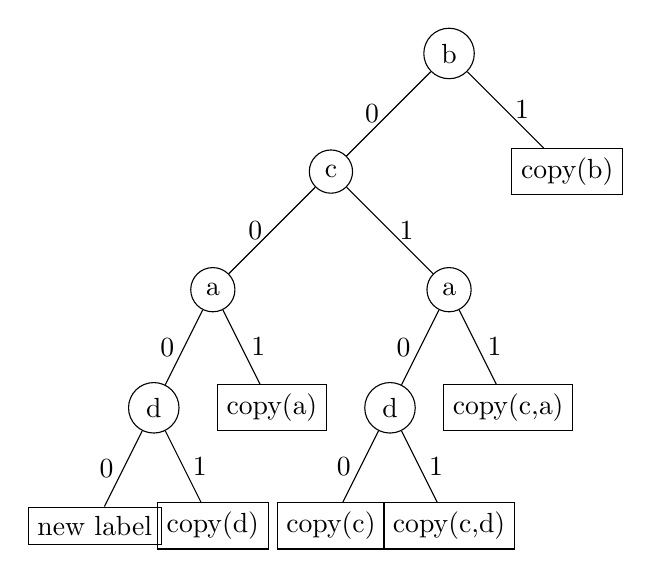
\begin{tikzpicture}[level distance=1.5cm,
  level 1/.style={sibling distance=3 cm},
  level 2/.style={sibling distance=3 cm},
  level 3/.style={sibling distance=1.5cm},
  level 4/.style={sibling distance=1.5cm}]
  \node[circle,draw] {b}
   child 
   {
    	node[circle,draw] {c}
      	child 
      	{
      	    	node[circle,draw] {a}
      	    	child
      	    	{
      	    		node[circle,draw]{d}
      	    		child
      	    		{
      	    			node[rectangle,draw]{new label}
      	    			edge from parent node[left,draw=none] {0}
      	    		}
      	    		child
      	    		{
      	    			node[rectangle,draw]{copy(d)}
      	    			edge from parent node[right,draw=none] {1}
      	    		}
      	    		edge from parent node[left,draw=none] {0}
      	    	}
      	    	child
      	    	{
      	    		node[rectangle,draw]{copy(a)}	
      	    		edge from parent node[right,draw=none] {1}
      	    	}
      	    	edge from parent node[left,draw=none] {0}
      	}
      	child 
      	{
      		node[circle,draw] {a}
      		child
      		{
      			node[circle,draw]{d}
      	    		child
      	    		{
      	    			node[rectangle,draw]{copy(c)}
      	    			edge from parent node[left,draw=none] {0}
      	    		}
      	    		child
      	    		{
      	    			node[rectangle,draw]{copy(c,d)}
      	    			edge from parent node[right,draw=none] {1}
      	    		}
      	    		edge from parent node[left,draw=none] {0}
      		}
      		child
      		{
      			node[rectangle,draw]{copy(c,a)}
      			edge from parent node[right,draw=none] {1}
      		}
      		edge from parent node[right,draw=none] {1}
      	}
      	edge from parent node[left,draw=none] {0}
    }
    child 
    {
    	node[rectangle,draw] {copy(b)}
    	edge from parent node[right,draw=none] {1}
    };
\end{tikzpicture}
\caption{Decision tree suggested in \em{CCLLRPC}}
\label{dtree}
\end{figure}
